\documentclass[a4paper, 11pt]{article}

\usepackage[slovene]{babel}
\usepackage[utf8]{inputenc}
\usepackage[T1]{fontenc}
\usepackage{lmodern}
\usepackage{amsmath}
\usepackage{amsfonts}
\usepackage{amssymb}
\usepackage{enumitem}
\usepackage{epsdice}
\usepackage{array}
\usepackage[table]{xcolor}
\usepackage{makecell}
\usepackage{hyperref}

\usepackage{geometry}
\geometry{
 a4paper,
 total={170mm,257mm},
 left=25mm,
 top=25mm,
 }

\newcolumntype{P}[1]{>{\centering\arraybackslash}p{#1}}

\begin{document}

\title{\textbf{\LARGE{Model napovedi odjema električne energije}} \\ Matematika z računalnikom 2023/24}
\author{Karolina Šavli}
\date{Maj 2024}

\maketitle

% =======================================================================================================================
% =======================================================================================================================


\section{Uvod}

Cilj projektne naloge je sestaviti model, ki bo napovedal odjem električne energije 
za celotni naslenji dan (za naslednjih $24$ ur). 

Celotna analiza je izvedena v programskem jeziku \href{https://www.python.org/}{Python}.



% =======================================================================================================================
% =======================================================================================================================


\section{Osnovna analiza časovne vrste}

\noindent Podjetje \href{https://gen-i.si/}{GEN-I} je v obliki excel razpredelnice pripravilo tabelo podatkov, sestavljeno iz sedmih stolpcev:
\begin{itemize}
    \item  \texttt{DateTimeStartUTC}: univerzalni koordinirani čas,
    \item  \texttt{DateTimeStartCET}: srednjeevropski čas,
    \item  \texttt{Odjem ACT}: neto odjem električne energije v kWh,
    \item  \texttt{Temperatura ACT}: dejanska temperatura, 
    \item  \texttt{Temperatura FC}: napovedana temperatura,
    \item  \texttt{Sevanje ACT}: dejansko sevanje in
    \item  \texttt{Sevanje FC}: napovedano sevanje. 
\end{itemize}

\begin{figure}[h!]
    \centering
    \caption{Tabela podatkov, 2021-2024}\par\medskip
    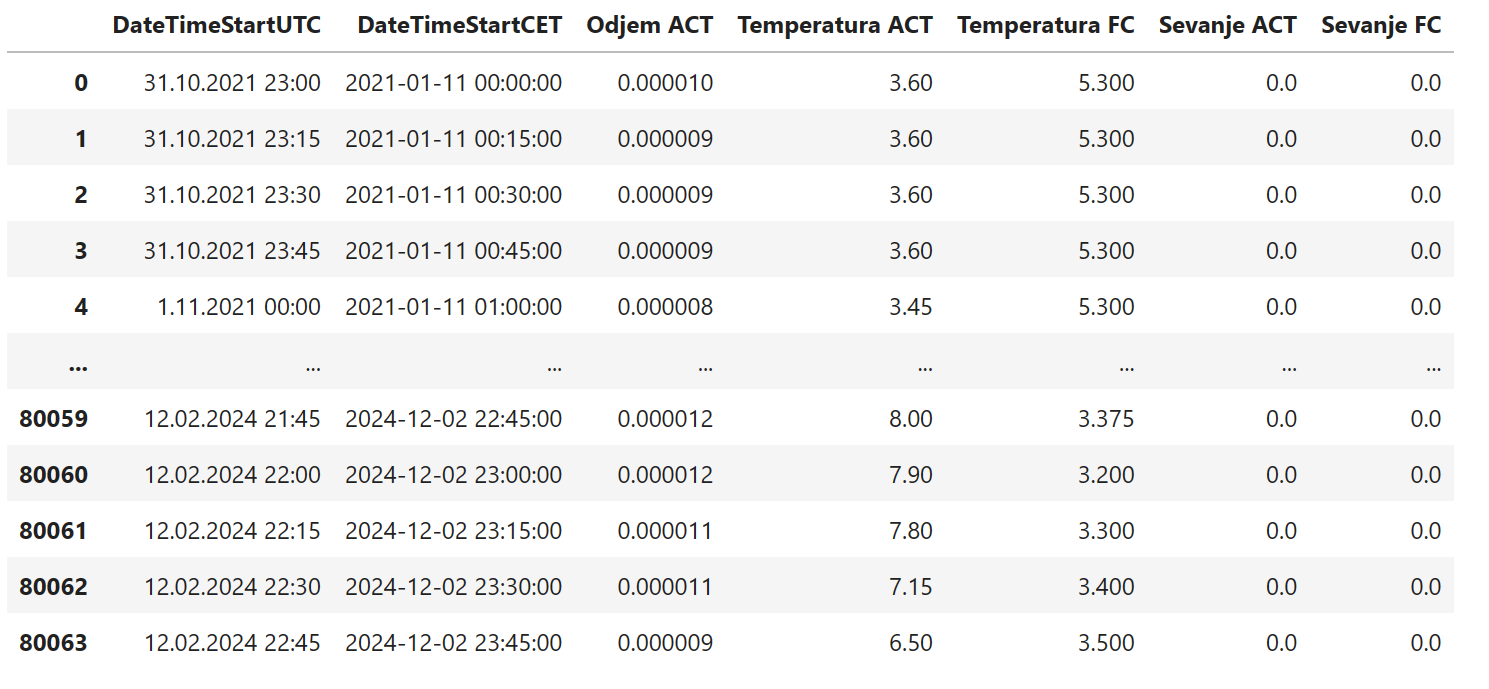
\includegraphics[width=0.9\textwidth]{tabela.png}
\end{figure}

\noindent V analizi sem uporabljala vse stolpce, razen stolpca \texttt{DateTimeStartUTC}, saj je v 
okviru časa bolj relavanten stolpec \texttt{DateTimeStartCET}. Podatki so podani za odboje od $1.~\text{novembra}~2021$ do $12.~\text{februarja}~2024$,
na vsakih $15$ minut. Tabela ima torej vsega skupaj $80064$ vrstic.

\begin{figure}[h!]
    \centering
    \caption{Odjem električne energije, 2021-2024}\par\medskip
    \label{fig:odjem_EE}
    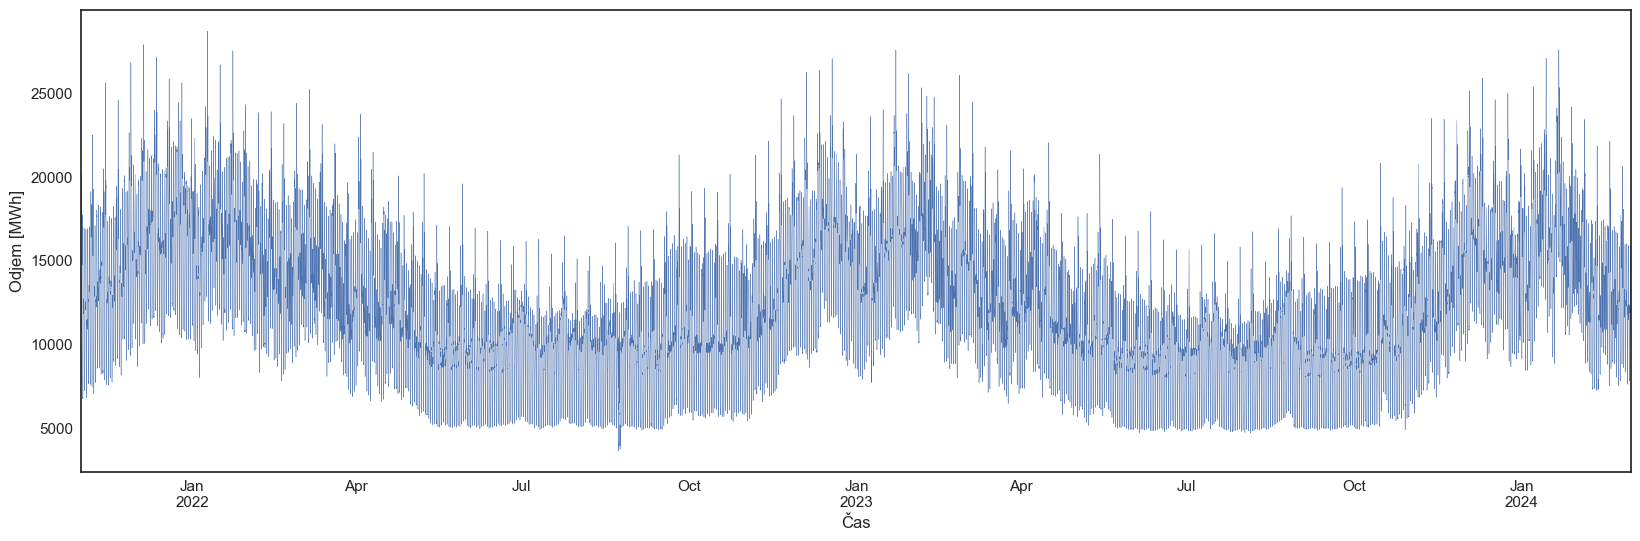
\includegraphics[width=0.9\textwidth]{odjem_EE.png}
\end{figure}

\noindent Slika~\ref{fig:odjem_EE} prikazuje odjem električne energije za obdobje od 
$1.~\text{novembra}~2021$ do $12.~\text{februarja}~2024$. 
Opaznoa je sezonskost; odjem je znatno večji jeseni in pozimi, zaradi povečane uporabe energije za ogrevanje in 
razsvetljevo, saj se število ur dnevne svetlobe podaljša. 

\begin{table}[!h]
    \centering
    \caption{Opisne statistike porabe električne energije, 2021-2024}\par\medskip
    \label{Tab:opisne_statistike}
    \begin{tabular}{l||l|l|l|l|l}
              & Min & Max & Povprečje & Mediana & Standardni odklon \\ \hline \hline
        Odjem [MWh] & 3629,32 & 28736,80 & 12240,53 & 11708,50 & 4167,98 \\ 
    \end{tabular}
\end{table}

\noindent S Tabele~\ref{Tab:opisne_statistike} preberemo, da je povprečna poraba električne energije gospodinjskih odjemalcev
okrog $12240{,}53 $ MWh, minimalna dosežena vrednost je $3629{,}32$ MWh, maksimalna pa $28736{,}80$ MWh. Vrednosti varirajo
okrog $4167{,}98$ MWh. \\

\noindent Odjem električne energije je med tednom najmanjši ponoči in se veča do viška okrog 18 ure. 
V soboto in nedeljo pa je prvi višek porabe dopoldne, drugi pa okrog 18 ure, kar je opazno s Slike~\ref{fig:odjem_teden}, ki prikazuje odjem 
električne energije v drugem tednu septembra 2023. Imamo torej tudi sezonskost na dnevni ravni.

\begin{figure}[h!]
    \centering
    \caption{Odjem električne energije po urah, drugi teden septembra 2023}\par\medskip
    \label{fig:odjem_teden}
    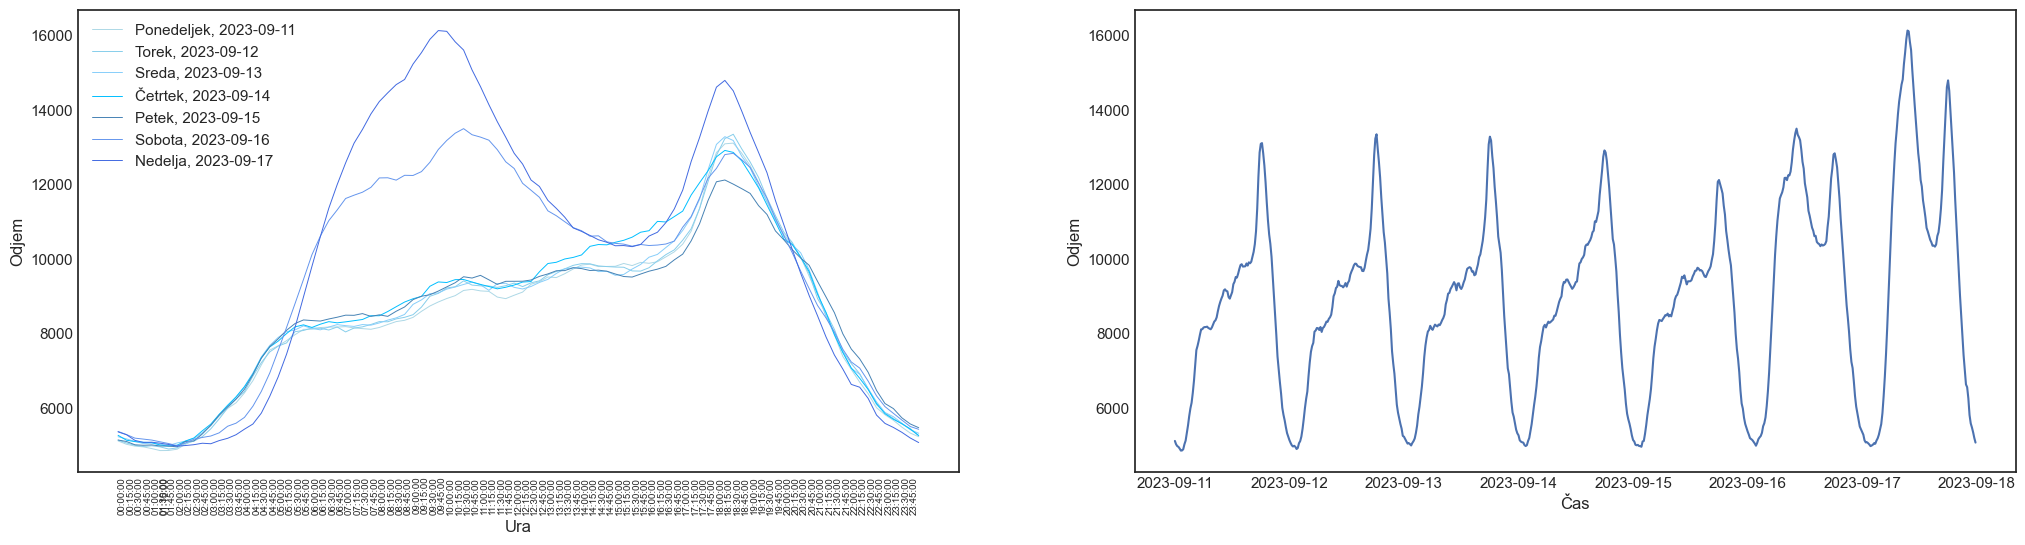
\includegraphics[width=0.9\textwidth]{odjem_teden.png}
\end{figure}

\noindent Zaključimo lahko, da je naša časovna vrsta visokofrekvenčna, ima sezonsko komponentno ter njeno povprečje ni konstantno.

% =======================================================================================================================
% =======================================================================================================================


\section{Napredna analiza}

\subsection{Izbira družine modelov}

ARIMA je model, ki pri napovedovanju zajame vzorce, trende in sezonskost podatkov s kombinacijo preteklih 
vrednosti, razlik in napak. Ker pa imamo v podatkih očitno sezonskost, lahko ARIMO nadgradimo v SARIMO, ki dodatno
upošteva še sezonske vzorce. Ta družina modelov ima težavo predvsem pri napovedih, ko ima časovna vrsta 
skozi čas spremembo variance. Da bo naše napovedovanje bolj učinkovito, bomo naš SARIMA nadgradili v 
model SARIMA-GARCH, saj se model GARCH uporablja ravno za modeliranje združevanja volatilnosti 
v podatke časovnih vrst.~\cite{ArimaGarch}


\subsection{Odstranitev sezonskosti in pridobitev stacionarnosti}

Da bomo lahko indentificiralni potencialne modele, moramo najprej originalno časovno vrsto (Slika~\ref{fig:odjem_EE})
narediti stacionarno. \\

\noindent Ker so naši podatki volatilni najprej naredimo \textbf{logaritmične donose} 
(ang. \emph{log returns}). Če z $W_t$ označimo originalno časovno vrsto odjema električne energije, so logaritmični donosi
definirani kot časovna vrsta $ Y_t = \ln \left( \frac{W_t}{W_{t-1}} \right) $. Slednja časovna vrsta je prikazana na
Slika~\ref{fig:log_returns}.

\begin{figure}[h!]
    \centering
    \caption{Logaritmični donosi odjema električne energije, 2021-2024}\par\medskip
    \label{fig:log_returns}
    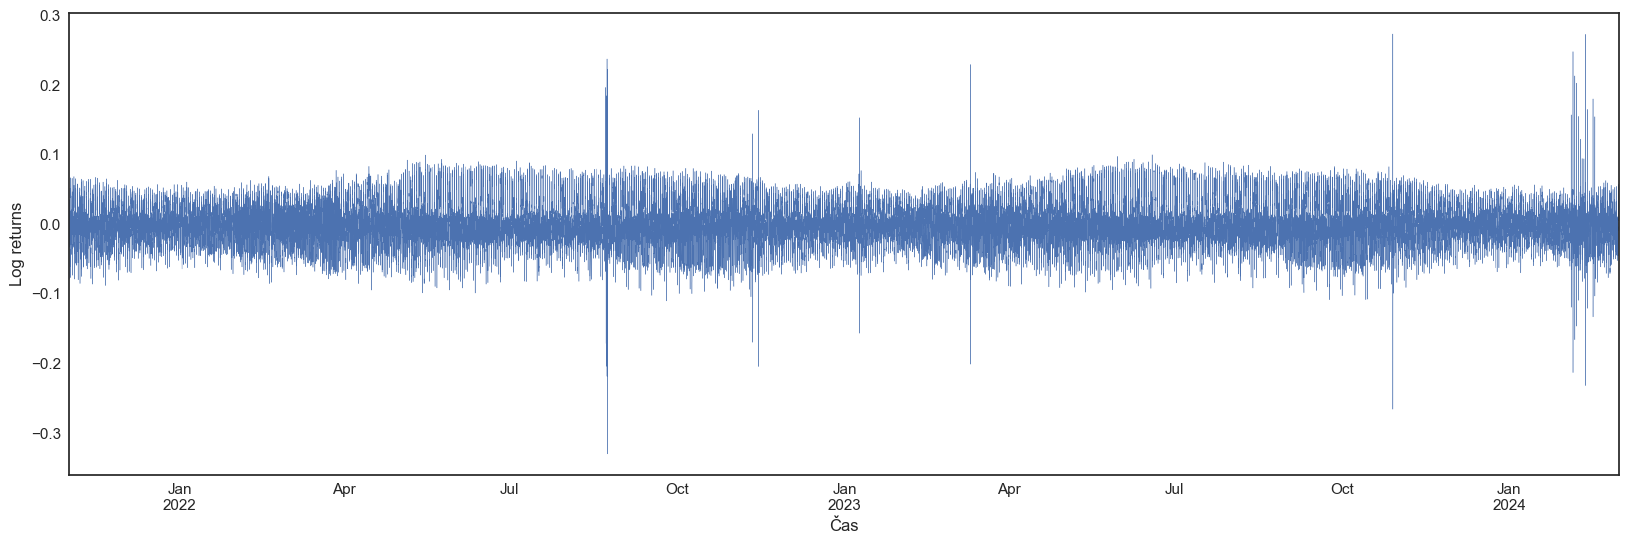
\includegraphics[width=0.9\textwidth]{log_returns.png}
\end{figure}

\noindent Slika~\ref{fig:log_returns_acf_pacf} prikazuje 
ACF (vzorčno avtokorelacijo) in PACF (vzorčna parcialna avtokorelacija) logaritmičnih donosov do odloga $1000$ (to je
malo manj kot dva tedna). Z grafov je očitno, da časovna vrsta ni stacionarna. Opazna je sezonska komponentna, in sicer $96$, 
kar je ravno en dan \footnote{Podatki so podani na $15$ minut in $15\,\text{min} \cdot 96 = 1440\,\text{min}$, kar je ravno en dan.}.

\begin{figure}[h!]
    \centering
    \caption{Vzorčna avtokorelacijska in parcialna avtokorelacija funkcija časovne vrste logaritmičnih donosov}\par\medskip
    \label{fig:log_returns_acf_pacf}
    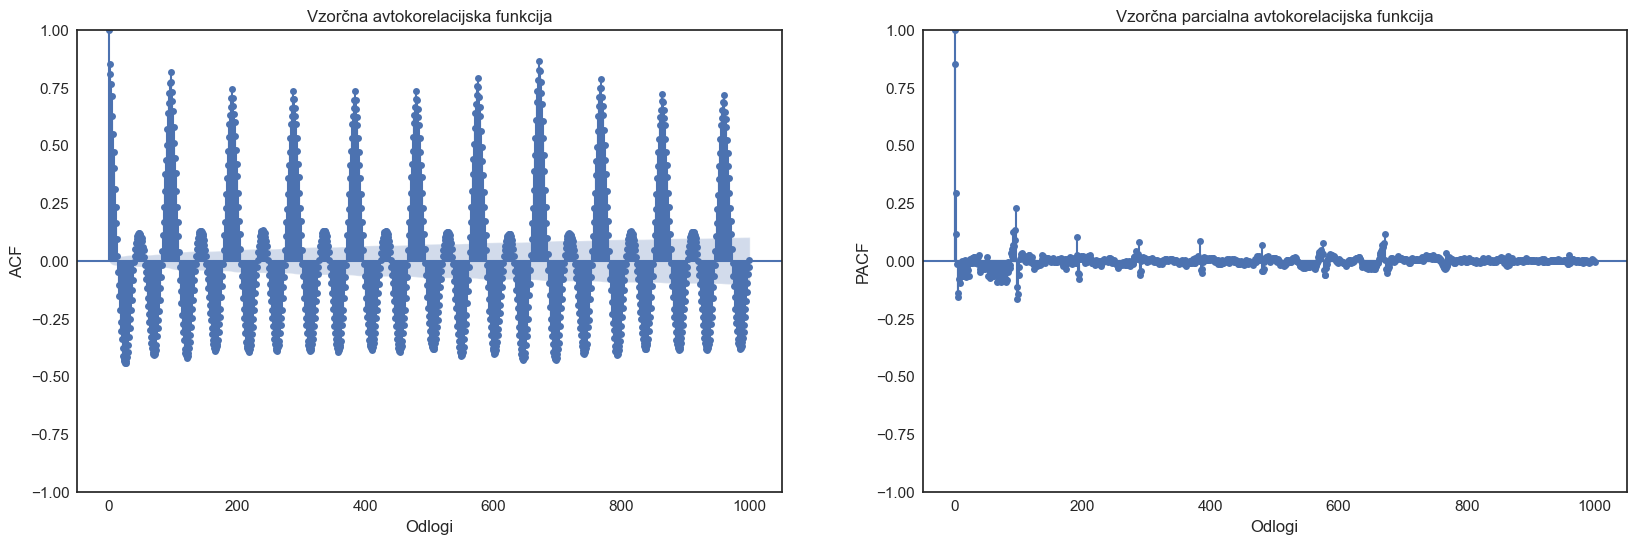
\includegraphics[width=0.9\textwidth]{log_returns_acf_pacf.png}
\end{figure}

\noindent Da dosežemo stacionarnost, se je potrebno sezonskosti znebiti, zato bomo podatke \textbf{sezonsko diferencirali}.
Nova časovna vrsta bo $Z_t = Y_t - Y_{t-96}$. Prikazana je na Slika~\ref{fig:ts_diff}, njeni ACF in PACF pa na Slika~\ref{fig:ts_diff_acf_pacf}.

\begin{figure}[h!]
    \centering
    \caption{Časovna vrsta po sezonskem diferenciranju, 2021-2024}\par\medskip
    \label{fig:ts_diff}
    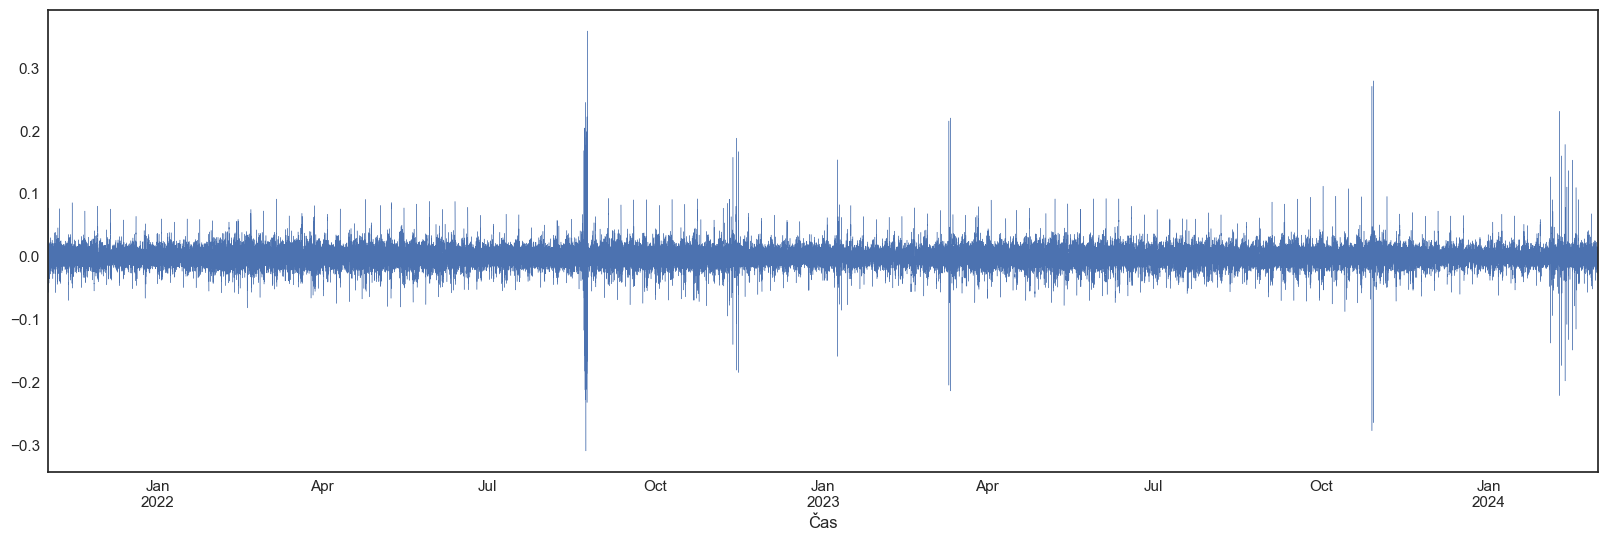
\includegraphics[width=0.9\textwidth]{ts_diff.png}
\end{figure}

\begin{figure}[h!]
    \centering
    \caption{Vzorčna avtokorelacijska in parcialna avtokorelacija funkcija časovne vrste po sezonskem diferenciranju}\par\medskip
    \label{fig:ts_diff_acf_pacf}
    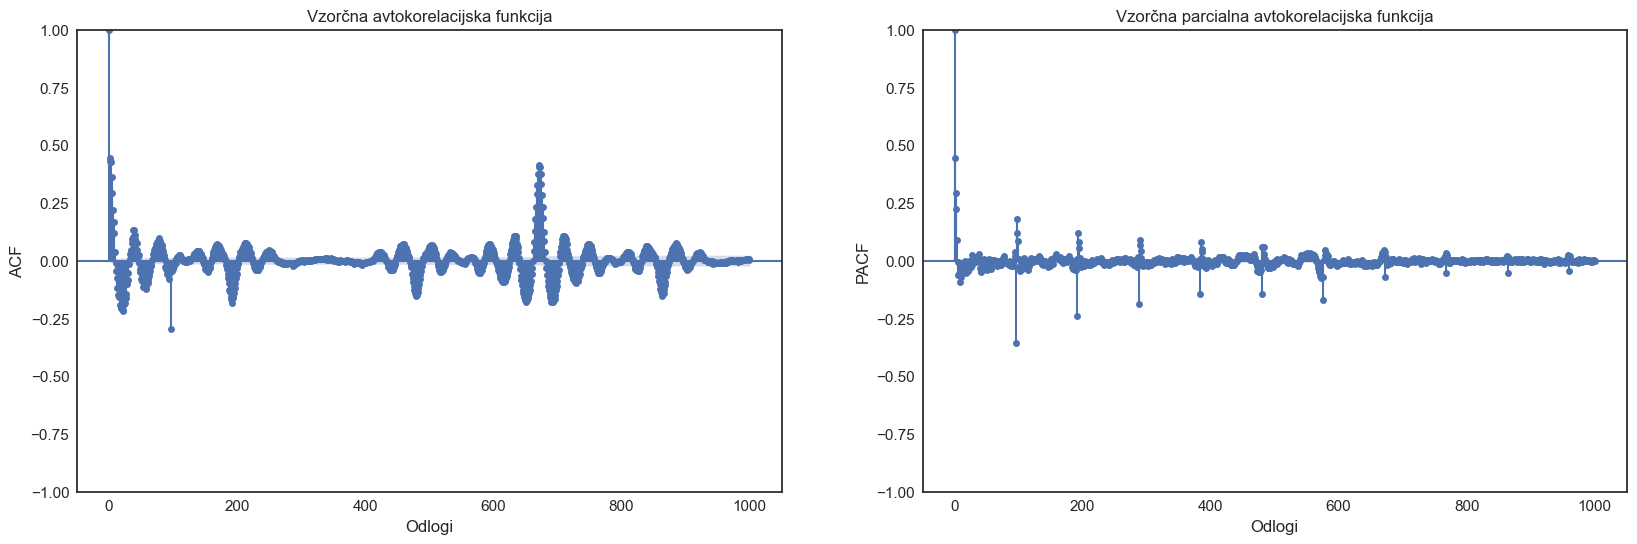
\includegraphics[width=0.9\textwidth]{ts_diff_acf_pacf.png}
\end{figure}

\noindent Na grafu ACF opazimo ponavljanje vzorca, kar pomeni, da časovna vrsta $Z_t$ še kar ni stacionarna. 
Še enkrat jo diferenciramo in dobimo vrsto $X_t = Z_t - Z_{t-1}$. 
Prikazana je na Slika~\ref{fig:ts_diff_2}, njeni ACF in PACF pa na Slika~\ref{fig:ts_diff_2_acf_pacf}.

\begin{figure}[h!]
    \centering
    \caption{Časovna vrsta po prvem nesezonskem diferenciranju, 2021-2024}\par\medskip
    \label{fig:ts_diff_2}
    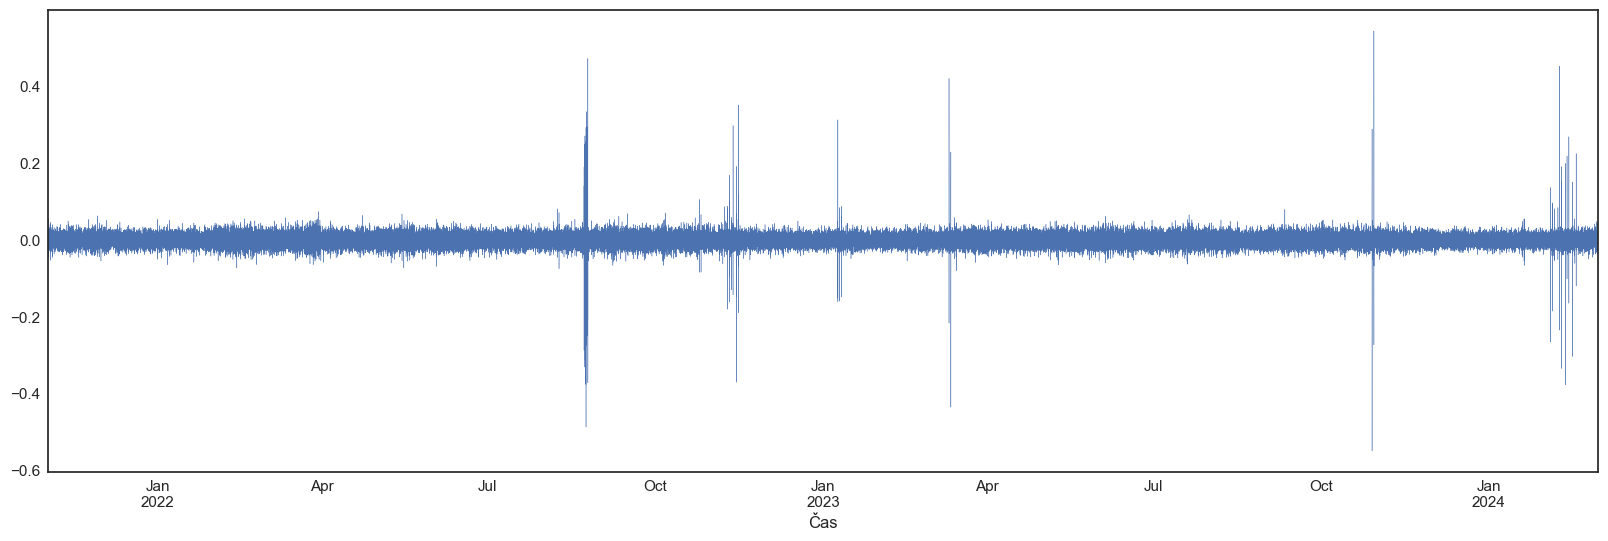
\includegraphics[width=0.9\textwidth]{ts_diff_2.png}
\end{figure}

\begin{figure}[h!]
    \centering
    \caption{Vzorčna avtokorelacijska in parcialna avtokorelacija funkcija časovne vrste po prvem nesezonskem diferenciranju}\par\medskip
    \label{fig:ts_diff_2_acf_pacf}
    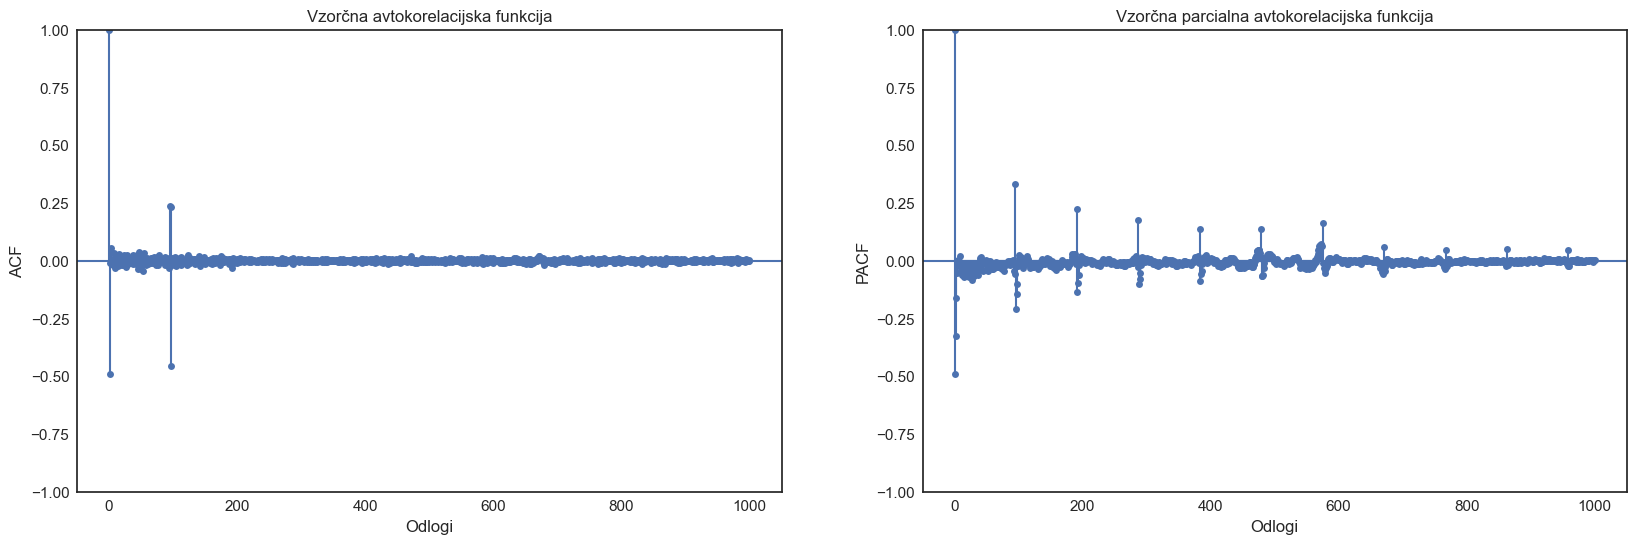
\includegraphics[width=0.9\textwidth]{ts_diff_2_acf_pacf.png}
\end{figure}

\noindent Dobljena časovna vrsta $X_t$ zgleda stacionarno in tudi formalni testi Augmented Dickey-Fuller (ADF), 
KPSS in Phillips-Perron potrdijo njeno stacionarnost. Časovna vrsta je torej primerna za izbero parametrov modela
SARIMA. 

\subsection{Identifikacija modela SARIMA}

\noindent Na podlagi ACF in PACF (Slika~\ref{fig:ts_diff_2_acf_pacf}) stacionarne časovne vrste $X_t$ izberimo parametre 
modela SARIMA(p, d, q)(P, D, Q)[S]. Kaj sploh predstavljajo ti parametri? Razdelimo jih lahko v dve skupini,
in sicer v skupino nesezonskih (p, d, q) in sezonskih (P, D, Q, S)~\cite{SARIMA_param}:

\begin{itemize}
    \item p \dots
    \item d \dots
    \item q \dots
    \item P \dots
    \item D \dots
    \item Q \dots
    \item S \dots
\end{itemize}

\noindent Ker smo časovno vrsto enkrat sezonsko diferencirali bo $\text{D} = 1$ in ker smo jo enkrat 
navadno diferencirali bo $\text{d} = 1$. Perioda je enaka $96$, torej je $\text{S} = 96$. \\

\noindent Za določitev sezonskih parametrov P in Q gledamokorelacije pri odlogih, ki so večkratniki periode S. Pri
PACF visoko korelacijo opazimo predvsem pri $96$ in $192$, nato pa se z vsako dodatno periodo manjša. Parameter P je torej 
$1$ ali več; predlagala bi $1$, $2$ ali $3$. 
Pri ACF pa je občutna korelacija zgolj pri $96$, zato vzamemo $\text{Q} = 1$. \\

\noindent Za lažjo določitev nesezonskih parametrov p in q bomo gledali ACF in PACF do prve periode (torej do odloga 96). 
Slednje je prikazano na Slika~\ref{fig:ts_diff_2_acf_pacf_do_100}. Tako iz PACF, kot tudi iz ACF, je opazna večja korelacija
pri prvih nekaj urah in v uri tik pred periodo. V modelu bomo zato zagotovo vključili prvih nekaj ur, saj le-te kažejo močan vpliv. \\

\begin{figure}[h!]
    \centering
    \caption{Vzorčna avtokorelacijska in parcialna avtokorelacija funkcija časovne vrste po prvem nesezonskem diferenciranju, odlogi do 100}\par\medskip
    \label{fig:ts_diff_2_acf_pacf_do_100}
    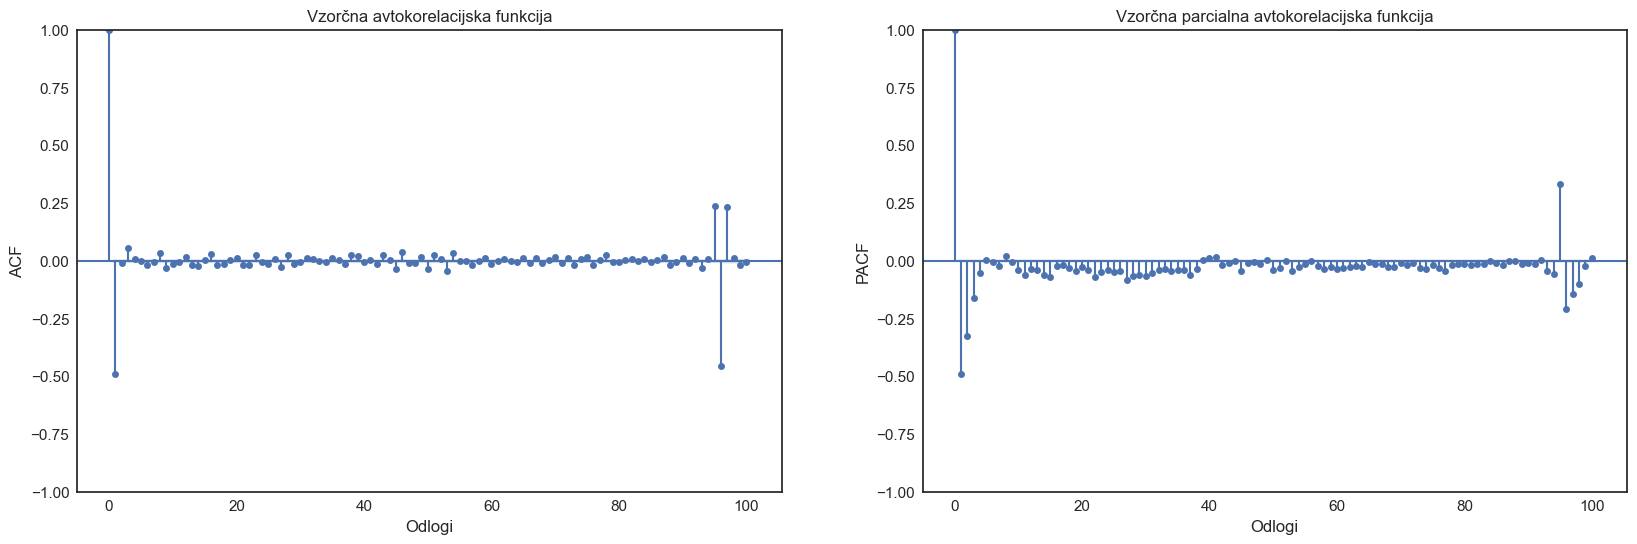
\includegraphics[width=0.9\textwidth]{ts_diff_2_acf_pacf_do_100.png}
\end{figure}


% =======================================================================================================================
% =======================================================================================================================


\section{Izbira modela}



% =======================================================================================================================
% =======================================================================================================================


\section{Zaključek}



% =======================================================================================================================
% =======================================================================================================================

\pagebreak

\bibliographystyle{abbrv}
\bibliography{literatura.bib}


\end{document}
